\section{Appendix C: Code Examples}

\subsection{Ageing Error Estimation}
\hypertarget{AgeingError}{}
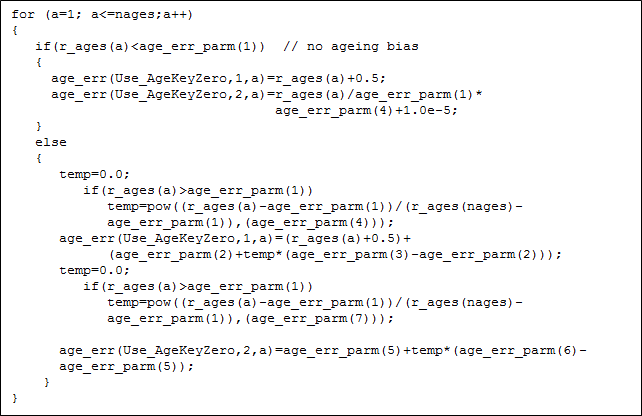
\includegraphics{age_error2}
The 7 parameters are:

\begin{itemize}
	\item age at which the estimated pattern begins (just linear below this age).  This is “start age”
	\item bias at start age (as additive offset from unbiased age’)
	\item bias at maxage (as additive offset from unbiased age’)
	\item power fxn coefficient for interpolating between those 2 values (value of 0.0 produces linear interpolation in the bias)
	\item stdev at age
	\item stdev at max age
	\item power fxn coefficient for interpolating between those 2 values
\end{itemize}


\subsection{Survival Based SRR Code}
\hypertarget{AppendixC}{Code} for the survival based recruitment is shown below:\\
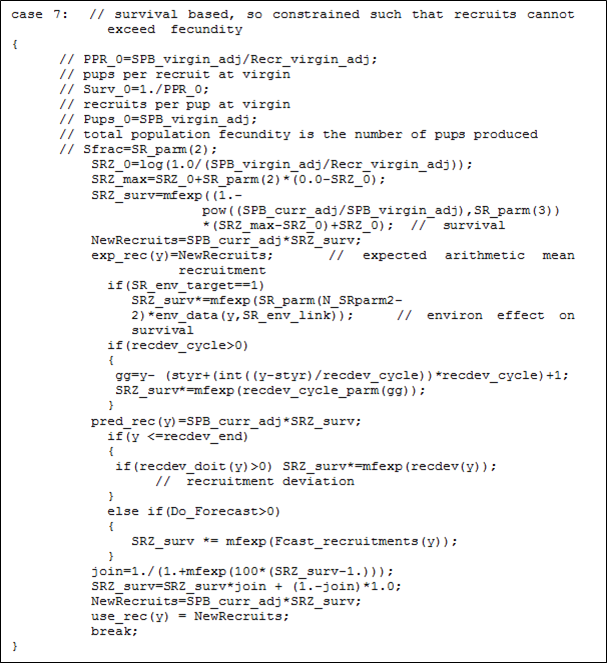
\includegraphics{survival_code2}

\subsection{Random Walk Selectivity: Pattern 17}
\hypertarget{RandWalkSelex}{}
	\begin{center}
		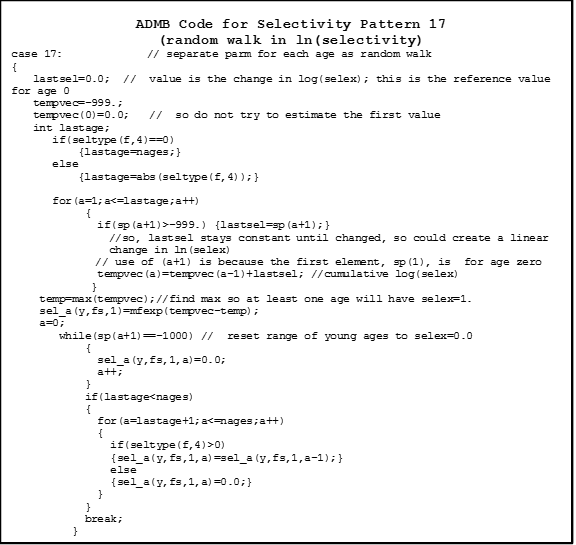
\includegraphics{Selex17_RandomWalk}
		\end{center}

\subsection{Cubic Spline Selectivity}
\hypertarget{CubicSpline}{}
	\begin{center}
		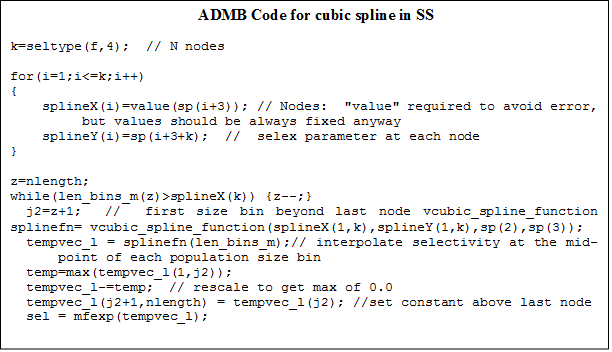
\includegraphics{CubicSplineCode}
	\end{center}